\documentclass[twocolumn,letterpaper]{article}

%encoding
%--------------------------------------
\usepackage[utf8]{inputenc}
\usepackage[T1]{fontenc}
\usepackage[french]{babel}

% mise en page
%--------------------------------------
\usepackage[margin=0.75in]{geometry}
\usepackage{titlesec}
\titlespacing*{\subsection}{0pt}{1.1\baselineskip}{\baselineskip}
\titlespacing*{\subsubsection}{0pt}{1.1\baselineskip}{\baselineskip}

% font
% --------------------------------------
\usepackage{lmodern}
\renewcommand{\familydefault}{\sfdefault}
\usepackage{mathpazo}

% custom sections
%--------------------------------------
\usepackage{titlesec}
\titleformat
{\section} % command
[block] % shape
{\bfseries\Large\itshape} % format
{\thesection} % label
{0.5ex} % sep: horizontal separation between label and title body
{ } % before-code
[\vskip-8pt\rule{0.49\textwidth}{1pt}] % after-code

\setlength
\parindent{0pt} % no indent

%packages
%--------------------------------------
\usepackage{tikz}
\usetikzlibrary{decorations.shapes}
\usepackage[many]{tcolorbox}
\usepackage{amsmath}
\usepackage{graphicx}% insert images
\usepackage{xcolor}

%snippets
%--------------------------------------
% REQUIRES:
% \usepackage{tikz}
% \usetikzlibrary{decorations.shapes}
% \usepackage[many]{tcolorbox}

% USAGE
% \begin{RoundBox}
%     test
% \end{RoundBox}

\newtcolorbox{RoundBox}{
    enhanced,
    arc=4pt,
    frame hidden,
    interior hidden,
    borderline={0.4pt}{0pt}{dashed},
}

\newcommand{\rbox}[1]{%
\begin{tcolorbox}[
    enhanced,
    arc=4pt,
    frame hidden,
    interior hidden,
    borderline={0.4pt}{0pt}{dashed}]
    #1
\end{tcolorbox}
}

%commands
%--------------------------------------
\newcommand{\pageRef}[2]{{\scriptsize \textcolor{blue}{C{#1}/S{#2}}}}
\newcommand{\pRef}[1]{{\scriptsize \textcolor{blue}{#1}}}

\title{GIA400}
\author{Hivers 2020 | Sophie Bernadin-Mercier}
\date{}

\begin{document}

\maketitle

\tableofcontents

\section{Fonctions TI}
$$tvmPV(N,i,A,F,[K],[M],[\emptyset,1])$$
$$tvmFV(N,i,P,A,[K],[M],[\emptyset,1])$$
$$tvmPMT(N,i,P,F,[K],[M],[\emptyset,1])$$
$$tvmI(N,P,A,F,[K],[M],[\emptyset,1])$$
$$tvmN(i,P,A,F/P)$$
$$npv(i,P_0,\{P_n,..\},\{f_n,...\})$$
$$iper(r,m,k)$$
$$ieff(r,c,k)$$
$$MIRR(ifin, ireinv, CFo, \{CF1..CFn\},\{f1..fn\})$$
$$IRR(P_0,\{f_1, f_2, .., f_n\},\{..\})$$
$$pvgl(n,i,a,g)$$
$$pvgg(n,i,a_1,g)$$

{\footnotesize *taux $i$ en \% }

\section{Stuff}
\begin{center}
\textbf{Valeur présente d'une perpétuité}
$$P=\frac{A}{i}$$

\textbf{Revenus}
\begin{equation*}
    \begin{split}
        Profits(\pi)&=Revenus - Couts\ totaux\\
        &=Revenus - CV - CF \\
        &=P*Q-CV*Q-CF\\    
    \end{split}
\end{equation*}
{\scriptsize P=Prix de vente\\Q=Quantité\\CV=Coûts variable\\CF=Coûts fixe}

\end{center}

\setcounter{section}{5}

\section{Financement}

\subsection{Obligations}

\rbox{
    \textbf{Valeur du coupon}
    $$C_\%=i_{periode}=\frac{i}{M}$$
    $$C_\$=A=C_\% *\ VN$$
    {\scriptsize
        $VN$ = valeur nominale (F)\\
        $i$ = taux nominal capitalisé du coupon\\
        $M$ = nombre de périodes par an\\
        \vskip3pt
        \textit{Exemple: i\% nominal composé semestriellement; i/2 pour avoir le taux semestriel}
    }
}

\rbox{
    \textbf{Valeur des intérêts (\$)}
    \begin{equation*}
        \begin{split}
        I_{periode} &=C\%\ *\ VN \\
        I_{annuel} &= I_{periode}*M \\
        I_{total\ par\ an} &= Nb * I_{annuel}
        \end{split}
    \end{equation*}
    {\scriptsize
        $i$ = taux du coupon
    }
}

\rbox{
    \textbf{Taux par période}
    \begin{equation*}
        \begin{split}
            i_{periode}&=tvmI(N,-P_{net},A,F) \\
            &=irr(-P_{net},\{A,F+A\},\{N-1,1\})
        \end{split}
    \end{equation*}
    \textbf{Taux annuel effectif}
    $$r=i_{nominal}=i_{periode}*M$$
    \textbf{Taux d'intérêt annuel effectif de l'obligation}\\
    {\scriptsize Rendement d'une obligation}
    $$K_{Obl\ brut}= i_{eff}=iper(r,M,1)$$
    {\scriptsize
        $N$ = nombre de périodes restantes(années * périodes par an)\\
        $M$ = 2 pour un semestre comme période
    }
}

\subsection{Coût de l'endettement}
Deux catégories: dettes et obligations

\subsection{Coût des capitaux propres}
\pageRef{6}{43}
L’entreprise devrait laisser espérer aux actionnaires, sur le flux monétaire réinvesti en leur nom dans l’entreprise, un rendement au moins égal à ce que ces actionnaires pourraient obtenir en investissant eux-mêmes leurs dividendes dans des entreprises comparables.

Cependant, contrairement au coût de la dette, le coût des capitaux propres ne s’observe pas directement. Il doit être inféré à partir du prix des actions.

\rbox{
    \textbf{Prix net par action ou obligation}
    \begin{equation*}
        \begin{split}
        P_{net} &=Prix_{courant} * (1 - f_c)\\
                &= Prix_{courant} - F_c
        \end{split}
    \end{equation*}
    {\scriptsize
        \textcolor{red}{* $F_c*(1-t)$: si déductible d'impôt}\\\vskip1pt
        $f_c$ = frais d'émission en \% \\
        $F_c$ = frais d'émission en \$
    }
}

\rbox{
    \textbf{Frais d'émission (\$)}
    $$ F_c = P_{courant} - P_{net}$$
    
    \textbf{Frais d'émission (\%)}
    $$ f_c = 1 - \frac{P_{net}}{P_{courant}}$$
    
    \textbf{Frais totaux}
    $$F_{total} = Nb * F_c$$
}
\rbox{    
    \textbf{Nombre d'actions ou obligations}
    \begin{equation*}
        \begin{split}
        Nb  &=\frac{\$ financement}{P_{net}} \\
            &=\frac{Valeur\ totale}{Valeur\ unitaire}
        \end{split}
    \end{equation*}
}

\rbox{
    \textbf{Valeur marchande}
    $$VM = Nb \cdot P_{marche}$$
}

\subsection{Le français c'est difficile}
{\small
\textbf{Frais brut}; avant impôts; frais associés à la nouvelle émission

\textbf{Financement par actions}; bénéfices non répartis

\textbf{Prix du marché}; s'échange sur le \textit{marché}; valeur unitaire;

\textbf{Prix d'émission}; se transigent à; prix courant; "prix de l'action"; cours actuel; prix actuel; s'échange \textit{actuellement};

\textbf{Valeur nominale}; enregistrés aux livres; valeur aux livres; valeur comptable; valeur unitaire; \textcolor{red}{\textit{*Distinction entre valeur totale et unitaire}}\\

\textbf{$D_0$}; dernier dividende annuel versé;

\textbf{$D_1$}; dividende à la fin de l'année courante; dividende la première année;

}

\clearpage

\begin{center}
\begin{tabular}{||c c c |c c| c||} 
    \hline
    Source de financement & Valeur MARCHANDE & Poids & Avant impôt & Après impôt & Pondéré* \\
     & ($V$\$) & ($W$\%) & ($K_{brut}$\%) & ($K_{net}$\%) & (\%) \\[0.5ex] 
    \hline\hline
    Emprunts & $V_{Dette}$ & $W_{D}$ & $K_D$ & $K_{D_{net}}$ & $Pondere$ \\
    \hline
    Obligation & $V_{Obl}$ & $W_{Obl}$ & $K_{Obl}$ & $K_{Obl_{net}}$ & $Pondere$ \\
    \hline
    \textbf{Dette totale} & $V_{Dette\ totale}$ & & & $K_{dette\ totale}$ & $Pondere_{dette}$ \\
    \hline
    \\
    \hline
    Bénéfices non répartis & $V_{BNR}$ & $W_{BNR}$ & $K_{BNR}$ & $K_{BNR_{net}}$ & $Pondere$ \\
    \hline
    Actions privilégiés & $V_{AP}$ & $W_{AP}$ & $K_{AP}$ & $K_{AP}$ & $Pondere$ \\
    \hline
    Actions ordinaires & $V_{AO}$ & $W_{AO}$ & $K_{AO}$ & $K_{AO}$ & $Pondere$ \\
    \hline
    \textbf{Capitaux Propres} & $V_{CP}$ & & & $K_{CP}$ & $Pondere_{CP}$ \\
    \hline
    \\
    \hline
    \textbf{TOTAL} & $V_{totale}$ & 100\% & & \textbf{CMPC} & $Pdr_{dette} + Pdr_{CP} $ \\ 
    \hline
\end{tabular}
\end{center}

\begin{RoundBox}
\pageRef{6}{40}
$$K_D = Cout\ avant\ impot$$
$$K_{D_{net}} = Cout\ apres\ impot = K_D * (1-t)$$
$$Pondere = K_{D_{net}}\ *\ Poids$$
{\scriptsize
* Pondération calculée en fonction de $K$ ou $K_{net}$
}
\end{RoundBox}

\begin{RoundBox}
    \pageRef{6}{48,P.636}
    \textbf{Coût de nouvelles actions ordinaires}\\
    $$K_{AO}=\frac{D_1}{P_0 - F_c}+g = \frac{D_1}{P_0(1-f_c)}+g$$
    {\scriptsize
    $p_0$ = Prix par action, prix du marché \\
    $D_1$ = $D_0(1+g)$ = dividende de la première année \\
    $g$ = Taux annuel de croissance du dividende \\
    $f_c$ = Frais d'émissions en \% du prix des actions \\
    $F_c$ = Frais d'émission en \$\\
    \textit{*Les frais peuvent être déductibles d'impôts (ce qui serait spécifié), ils sont alors réduits de la valeur de l'impôt: $F_c net = F_c * (1-t)$}
}
\end{RoundBox}

\begin{RoundBox}
\pageRef{6}{51,P.636}
\textbf{Coût des actions privilégiées}\\
$$K_{AP}=\frac{D^*}{P^*-F_c}=\frac{D^*}{P^*(1-f_c)}$$
{\scriptsize
    $P^*$ = Prix actuel des actions, prix d'émission \\
    $D^*$ = Dividende fixe annuel \\
    $f_c$ = Frais d'émissions en \% du prix des actions \\
    $F_c$ = Frais d'émission en \$\\
    \textit{*Les frais peuvent être déductibles d'impôts, ils sont alors réduits de la valeur de l'impôt: $F_c net = F_c * (1-t)$}
}
\end{RoundBox}

\begin{RoundBox}
\pageRef{6}{51}
\textbf{Coût des bénéfices non répartis}\\
$$K_{BNR}=\frac{D_1}{P_0}+g$$
{\scriptsize
    $p_0$ = Prix par action, cours actuel de l'action \\
    $D_1$ = $D_0(1+g)$ = dividende de la première année \\
    $g$ = Taux annuel de croissance du dividende en \%
}
\end{RoundBox}

\newpage
\vspace*{5.75cm}

\begin{RoundBox}
\pageRef{6}{36}
\textbf{Moyenne pondérée du coût de l'endettement après impôt}
$$k_{dette\ totale}=W_D * K_D * (1 - t) + W_{obl}* K_{obl} * (1 - t)$$
{\scriptsize
    $W_D$ = fraction de la dette totale financée par un prêt à terme\\
    $K_D$ = taux d'intérêt sur le prêt à terme\\
    $W_{obl}$ = fraction de la dette totale financée par les obligations\\
    $K_{obl}$ = taux d'intérêt effectif sur les obligations\\
    $t$ = taux d'impôt marginal de l'entreprise
    \\\\
\textit{On doit aussi éventuellement tenir compte des frais d'émission des obligations.}
}
\end{RoundBox}


\begin{RoundBox}
\pageRef{6}{58}
\textbf{Moyenne pondérée du coût des capitaux propres}\\
$$K_{CP}=W_{BNR}*K_{BNR}+W_{AO}*K_{AO}+W_{AP}*K_{AP}$$
{\scriptsize
    $W_{BNR}$ = fraction des CP financés par les BNR \\
    $W_{AO}$ = fraction des CP financés par les actions ordinaires \\
    $W_{AP}$ = fraction des CP financés par les actions privilégiées \\
    $W_{BNR}+W_{AO}+W{AP}=1$
}
\end{RoundBox}


\begin{RoundBox}
\pageRef{6}{62}
\textbf{Coût moyen pondéré du capital}\\
$$CMPC=\frac{V_{Dette\ totale}}{V_{Totale}}*K_{Dette\ totale} + \frac{V_{CP}}{V_{Totale}}*K_{CP}$$
$$=Pondere_{dette} + Pondere_{CP}$$
\end{RoundBox}

\clearpage

\section{Analyse de projets}

\subsection{Délai de récupération}
\pageRef{7}{P.275} Méthode servant à déterminer \textit{à quel moment} d'un projet le seuil de rentabilité est atteint.\\

    \pageRef{7}{15}
    \textbf{Inconvénients}\\
        - Ne mesure pas la rentabilité d'un projet sur sa durée de vie totale.\\
        - Ne fournit pas une mesure de rentabilité directement comparable au coût du capital.\\
        - En tant que critère de sélection, la période de récupération maxiamle est purement arbitraire et subjective et élimine souvent des projets créateurs de valeur pour l'entreprise (dont le rendement est supérieur au coût du capital)
    \subsubsection{Sans actualisation}
    \begin{RoundBox}
        $$DR=annee\ n^* +\frac{Ce\ qui\ reste\ annee\ n}{Flux\ a\ l'annee\ n+1}$$
        \begin{footnotesize}
            * Année avant que "ce qui reste" atteint 0
        \end{footnotesize}
    \end{RoundBox}
    \textbf{Inconvénients:} Ne tient pas compte de l’influence du temps sur la valeur de l’argent

\subsubsection{Avec actualisation}
    \begin{RoundBox}
    $$Flux\ actualise = \frac{flux}{(1 + taux\ de\ rendement^*)^{annee}}$$
    $$DR=annee\ n +\frac{Ce\ qui\ reste\ annee\ n}{Flux\ actualise\ a\ l'annee\ n+1}$$
    \begin{footnotesize}
    * \% du taux de rendement en décimale
    \end{footnotesize}
    \end{RoundBox}

\subsection{Valeur actualisée nette équivalente (PE) \textcolor{red}{\textit{(Méthode du flux monétaire)}}}
    \pageRef{7}{P.275} Méthode d'équivalence qui convertit les flux monétaires d'un projet en une valeur nette.\\
    
    \noindent\fbox{%
            \parbox{0.45\textwidth}{%
            \begin{center}
                Si \textbf{PE > 0}, on accepte l’investissement\\
                Si \textbf{PE = 0}, on reste indifférent à l’investissement\\
                Si \textbf{PE < 0}, on rejette l’investissement
            \end{center}
            }%
        }\\
    \begin{RoundBox}
        $$VAN=PE=npv(i,-P_0,\{f_1, f_2, .., f_n\})$$\\
        \textbf{Gradient linéaire} (constant chaque année)
        $$PE=pvgl(n,i,A_1,g_\$)$$
        \textbf{Gradient géométrique} (\% de l'année précédente)
        $$PE=pvgg(n,i,P_0,g_\%)$$
        {\scriptsize
            $f$ = flux (actualisé ou non) à l'année 1 à n\\
            $i$ =  taux d'intérêt ou TRAM
        }
    \end{RoundBox}
    \noindent\fbox{%
        \parbox{0.45\textwidth}{%
        \begin{center}
            Si \textbf{PE(TRAM) > 0}, on accepte l'investissement\\
            Si \textbf{PE(TRAM) = 0}, indifférent à l'investissement\\
            Si \textbf{PE(TRAM) < 0}, on rejette l'investissement
        \end{center}
        }%
    }
    
\subsection{Valeur future nette équivalente (FE)}
    \pageRef{7}{P.275} Méthode d'équivalence qui convertit les flux monétaires d'un projet en une valeur future nette.
    \begin{RoundBox}
        $$FE(TRAM)=tvmFV(n, TRAM,-PE(TRAM),0)$$
        {\scriptsize
            $f$ = flux (actualisé ou non) à l'année 1 à n
        }
    \end{RoundBox}
    \noindent\fbox{%
        \parbox{0.45\textwidth}{%
        \begin{center}
            Si \textbf{FE(TRAM) > 0}, on accepte l’investissement\\
            Si \textbf{FE(TRAM) = 0}, indifférent à l’investissement\\
            Si \textbf{FE(TRAM) < 0}, on rejette l’investissement
        \end{center}
        }%
    }

\subsection{Valeur annuelle équivalente (AE)}
    \pageRef{7}{P.275} Méthode d'équivalence qui convertit les flux monétaires d'un projet en une valeur annuelle nette.
    \begin{RoundBox}
        {\small $$AE(TRAM)=tvmPMT(n, TRAM,-PE(TRAM),0)$$}
        {\scriptsize
            $f$ = flux (actualisé ou non) à l'année 1 à n
        }
    \end{RoundBox}
    \noindent\fbox{%
        \parbox{0.45\textwidth}{%
        \begin{center}
            Si \textbf{AE(TRAM) > 0}, on accepte l’investissement\\
            Si \textbf{AE(TRAM) = 0}, indifférent à l’investissement\\
            Si \textbf{AE(TRAM) < 0}, on rejette l’investissement
        \end{center}
        }%
    }

\subsection{Taux de rendement interne (TRI)}
    \pageRef{7}{P.253} Rendement du capital investi.

    \pageRef{7}{P.275} Méthode qui calcule le taux d'intérêt gagné sur les fonds à l'intérieur d'un projet.
    \begin{RoundBox}
        $$TRI=IRR(-P_0,\{f_1, f_2, .., f_n\},\{..\})$$
        {\scriptsize
            $f$ = flux (actualisé ou non) à l'année 1 à n
        }
    \end{RoundBox}
    \noindent\fbox{%
        \parbox{0.45\textwidth}{
        \begin{center}
            Si \textbf{TRI > TRAM}, on accepte l’investissement\\
            Si \textbf{TRI = TRAM}, indifférent à l’investissement\\
            Si \textbf{TRI < TRAM}, on rejette l’investissement
        \end{center}
        }
    }
    \subsubsection{Pourquoi rendement interne?}
        On parle de rendement « interne » car le calcul du TRI suppose que l’on peut réinvestir les flux monétaires du projet et obtenir un rendement égal au TRI.
    
    \subsubsection{TRIM}
    Une hypothèse plus réaliste serait que les flux monétaires du projet peuvent être réinvestis à un taux de rendement différent du TRI, comme, par exemple le TRAM. Le calcul du taux de rendement sous cette hypothèse est appelé le taux de rendement interne modifié (TRIM)
    $irr(-100,{0,279},{4,1}) = 22.78\%$
    \begin{RoundBox}
    $$TRIM=(\frac{FE(flux\ positifs)}{-PE(flux\ negatifs)})^{1/N}-1$$
    $$=MIRR(ifin, ireinv, CFo, \{CF1..CFn\},\{f1..fn\})$$
    \end{RoundBox}

\subsection{TRAM}
    \textbf{Choix du taux de rendement minimal acceptable}\\
    \pageRef{7}{P.641,\textbf{P.657}}
    Sans limite de capital, le choix du TRAM est dicté par la disponibilité des données de financement.\\
    
    1. Si les calendriers exacts de financement par emprunt et de remboursement de la dette sont connus, méthode du flux monétaire net des capitaux propres. TRAM serait donc le coût des capitaux propres $i_e$.\\
    
    2. Si aucun mode de financement précis, déterminer les flux monétaires après impôt sans intégrer de flux monétaires d'endettement. On utilise alors le coût marginal du capital ($k$) en tant que TRAM.
    
\subsection{Coût annuel total (AEC)}
    \pageRef{7}{41}
    Pour évaluer le coût annuel de l’entreprise, ou pour trouver le coût annuel dans le cas d’un projet par dépenses, nous utilisons l’AEC. 
    Valeur actualisée aujourd'hui de toutes nos dépenses.
    \textit{Coût à chaque année pour faire marcher le projet.}
        \begin{RoundBox}
        $$AEC=OC+RC$$
        \end{RoundBox}
    \noindent\fbox{%
        \parbox{0.45\textwidth}{
        \pageRef{7}{46} Rentabilité de l'achat d'un équipement
        \begin{center}
            Si \textbf{AEC > Revenus}, on rejette\\
            Si \textbf{AEC = Revenus}, indifférent\\
            Si \textbf{AEC < Revenus}, on accepte
        \end{center}
        }
    }

\subsubsection{Recouvrement en capital (RC)}
    \pageRef{7}{42} Coûts annuels équivalents en capitaux
    \begin{RoundBox}
        $$RC(i)=tvmPMT(N,i,P,-S)$$
        $$S=tvmFV(N,i,-P,RC(i))$$
        {\scriptsize
        $N$ = nombre d'années de vie \textbf{utile}\\
        $i$ = taux, potentiellement le TRAM\\
        $P$ = valeur de l'achat\\
        $S$ = prix de revente, valeur de récupération
        }
    \end{RoundBox}

\subsubsection{Coût d'opération (OC)}
    \pageRef{7}{42} Coûts annuels équivalents d'opération et d'entretien.

    Calculer l'AE des coûts d'opération.
    
\subsubsection{Exemple d'un projet par dépense}
\pRef{Solutionnaire TP8/S16}
    $$RC = tvmPmt(n,TRAM, (+)P_0, (-)S)$$
    {\footnotesize
        $n$: Durée de vie utile de l'équipement\\
        $P_0$: achat d'un équipement\\
        $S$: Prix de revente\\
    }
    \hrule
    $$PE = pvgg(n,TRAM,(-)P_0,g_\%)$$
    $$OC = tvmPmt(n,TRAM,PE,0)$$
    \hrule
    $$AEC = RC + OC$$

\subsubsection{Exemple d'un projet par revenu}
\pRef{Solutionnaire TP7/S17}
    $$RC=tvmPmt(n,TRAM,(-)P_0, (+)S)$$
    \hrule
    $$PE=pvgl(n,TRAM,A_1,g_\$)$$
    {\footnotesize
        $A_1$: Flux monétaire net de la première année\\
    }
    $$A=tvmPmt(n,TRAM,(-)PE,0)$$
    \hrule
    $$AE=(-)RC+A$$

\clearpage

\section{Projets mutuellement exclusifs}

\subsection{Analyse de remplacement}
\pageRef{8}{70}
- Les \textbf{coûts irrécupérables} qui ne doivent pas être considérés.\\
- Les \textbf{coûts d’exploitation} peuvent être considérés que dans la mesure où ils changeraient avec une nouvelle machine.\\
- La \textbf{valeur marchande actuelle} (non la valeur de reprise donnée par un fournisseur) et l’estimation actuelle de la valeur de récupération sont toujours pertinentes dans l’analyse du défenseur.

\subsubsection{Approche de comparaison}
- Le défenseur: l’équipement déjà en fonction\\
- L’aspirant: le nouvel équipement

\subsubsection{Deux méthodes}
- Flux monétaire $PE$\\
- Coût d’opportunité (ou coût d’option) $AEC$

\subsection{Comparaison de projets \textcolor{red}{\textit{(Méthode différentielle)}}}
On peut classer des projets selon leur TRI uniquement si l’investissement est identique.

Projet le plus cher - Projet le moins cher.\\

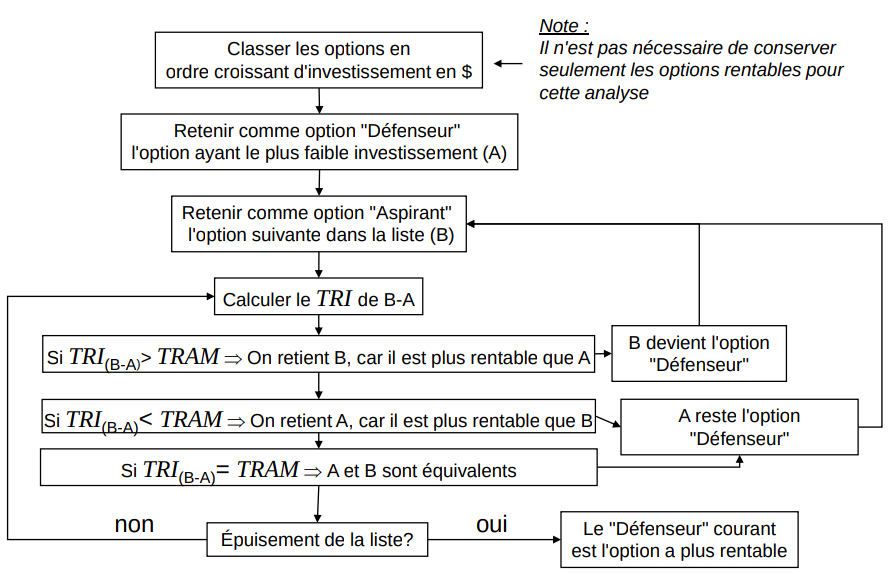
\includegraphics[scale=0.5]{images/analyse_differentielle.png}
\clearpage

\setcounter{section}{9}

\section{Analyse de rentabilité de projets après impôt}
\subsection{Qu’est-ce qu’un bien amortissable?}
\begin{enumerate}
    \item Un bien utilisé dans le cadre d’activités économiques ou détenu pour produire des bénéfices. • Principe fiscal important : une activité ou un amortissement sur un bien n’ayant aucune chance de produire des bénéfices n’est pas déductible aux fins d’impôt.
    \item Un bien ayant une vie utile définissable et supérieure à une année.
    \item Un bien qui s’use, se détériore, perdant ainsi de la valeur. • Amortissable : équipements, matériel roulant, bâtiments. • Non amortissable : terrains.
\end{enumerate}


\subsection{Coût amortissable}
\subsubsection{Principes comptables}
- Toutes les dépenses engagées pour acquérir et mettre en service sont amortissables.

- L’amortissement commence seulement lorsque le bien entre effectivement en service.


\subsection{Amortissement comptable}
- « Rapprocher » le mieux possible le coût d’un bien des revenus générés par ce bien.

- Utilisé dans les états financiers publiés dans les rapports annuels, les états financiers internes.

\subsection{Amortissement fiscal}
- Amortissement permis par l’agence du revenu du Canada (ARC) et Revenu Québec en vue du calcul de la déduction pour amortissement (DPA).

- En général, permet un amortissement plus rapide que l’amortissement comptable au début de la vie d’un bien. Ceci encourage l’investissement par les entreprises.

- Le gain fiscal ainsi réalisé (qui est en fait une subvention gouvernementale) est rapporté à la rubrique « Impôts reportés » au bilan.

\clearpage
\newcommand{\entry}[3]{\textbf{#1}\markboth{#1}{#1}\ {\scriptsize \textcolor{blue}{#2}} \ $\bullet$\ {#3}}

\section{Glossaire}
{\small
\subsection{Notes de cours}
\entry
{Actions ordinaires}
{C6/S43,P.622}
{Donnent droit à une participation aux bénéfices, proportionnelle au nombre d’actions détenues sur le total en circulation; Droit de vote aux assemblées : élection du conseil d’administration, nomination des vérificateurs externes.}

\entry
{Actions privilégiées}
{C6/S43,P.622}
{Priorité sur les actions ordinaires pour le paiement de dividendes; Dividende fixé à l’avance en \% de la valeur nominale.}

\entry
{Capitaux propres}
{P.621}
{Valeur d'une entreprise en sus de sa dette totale. Correspont aux droits que détiennent les actionnaires ordinaires et privilégiés sur l'entreprise.}

\entry
{Coût de l'endettement après impôt}
{C6/S36}
{Moyenne pondérée du coût aprèes impôts de chaque source d'endettement.}

\entry
{Coût des capitaux propres}
{C6/S42, P.657}
{Indice composé reflétant le coût des fonds obtenus de diverses sources. Rendement qu’il faut laisser espérer aux actionnaires pour pouvoir utiliser leur capital. Deux sources de rendement espéré pour les actionnaires: dividendes en espèces et/ou l’appréciation de la valeur de l’action, provenant du réinvestissement du flux monétaire non distribué dans les projets de l’entreprise.}

\entry
{Coût amortissable du bien à déprécier}
{C10/S8}
{Montant sur lequel les déductions pour amortissements sont calculées.\\\textbf{\textit{Il peut comprendre}} : • Les coûts des études d’ingénierie; • Le coût d’acquisition du bien; • Le coût de transport vers le site; • Le coût de préparation du site; • Le coût d’installation; • Et tout autre coût nécessaire pour rendre le bien fonctionnel\\\textbf{\textit{Il faut déduire de ces coûts}} : • La valeur de reprise d’un équipement existant que le nouvel équipement remplace. • Les crédits d’impôt, et autres subventions, offerts pour certains investissements.}

\entry
{Coût opérationnel (OC)}
{C7/S41}
{Coût annuel pour faire « fonctionner » la machine/projet}

\entry
{Délai de récupération}
{P.275}
{Méthode servant à déterminer \textit{à quel moment} d'un projet le seuil de rentabilité est atteint.}

\entry
{Dividendes}
{P.622}
{Revenu net d'une entreprise après le paiement des dividendes sur les actions privilégiées peut être versé aux actionnaires ordinaires sous la forme de dividendes ou réinvesti dans l'entreprise. Montant déterminé par le conseil d'administration.}

\entry
{Financement par actions}
{P.657}
{Utilise les bénéfices non répartis ou les fonds obtenus par l'émission d'actions pour financer un investissement.}

\entry
{Financement par emprunt}
{P.657}
{Utilise les fonds obtenus au moyen de prêts ou d'obligations émises pour financer un investissement.}

\entry
{Fonds empruntés}
{C7/S34}
{}

\entry
{Fond de placement commun}
{C7/S31}
{On peut voir la trésorerie de l’entreprise comme un fonds d’investissement rapportant au moins le TRAM. (si c’était moins que le TRAM, l’argent devrait être redistribué aux actionnaires!)}

\entry
{Obligations}
{C6/S15,P.182,P.194,P.627}
{Titre de créance donnant droit à des intérêts fixes(coupon) périodiques et au remboursement de la valeur nominale à maturité. Structure de financement très couteuse mais intéressante. Peut être émis par le fédéral, provincial, municipal ou grosses entreprises privées.\\Le prix de l'obligation s'ajuste au taux d'intérêt en vigueur sur le marché au moment précis de l'émission.}

\entry
{Obligation à coupon zéro}
{Solutionnaire TP6/S31}
{Obligation dont tous les coupons ont été enlevés, donc aucune annuité.}

\entry
{Obligation émise au pair}
{C6/S31}
{Obligation achetée à sa valeur nominale (généralement 1000\$).
\\ \textit{Taux du coupon = taux d'intérêt en vigueur sur le marché}}

\entry
{Obligation avec prime d'émission}
{C6/S31}
{Obligation achetée à un prix supérieur à sa valeur nominale (P > 1000\$).
\\ \textit{Taux du coupon > taux d'intérêt en vigueur sur le marché}}

\entry
{Obligation avec escompte d'émission}
{C6/S31}
{Obligation achetée à un prix inférieur à sa valeur nominale (P < 1000\$).
\\ \textit{Taux du coupon < taux d'intérêt en vigueur sur le marché}}

\entry
{Option Zéro ou Nulle}
{C8/S3}
{L'option de ne rien faire, c'est-à-dire de ne retenir aucune des options (statu quo). • Peut être une option en soi, avec un flux monétaire défini ou • Le flux des autres options peuvent être définis relativement à l'option Zéro, c’est-à-dire par analyse du flux monétaire différentiel entre les autres options et l’option Zéro.}

\entry
{Période de récupération}
{C7/S10}
{Méthode basée sur le temps nécessaire pour que les flux monétaires nets générés par le projet équivalent le montant de l’investissement}

\entry
{Projets indépendants}
{P.650}
{Lorsque l'on peut accepter ou rejeter sans que cela affecte la décision d'accepter ou rejeter un autre projet indépendant.}

\entry
{Projets dépendants conditionnels}
{P.650}
{Lorsque l'acceptation de l'un nécessite l'acceptation d'un autre.}

\entry
{Projets ou options mutuellement exclusifs}
{C8/S3}
{Acceptation de un entraine le rejet des autres. Toutes les options visent l'atteinte du même objectif, donc le choix de l'une d'entre elles élimine les autres par le fait même, même si elles sont rentables.}

\entry
{Projet par dépense}
{}
{On utilise l'AEC. L'objectif n'est pas de faire du profit.}

\entry
{Projet par revenu}
{}
{On utilise l'AE}

\entry
{Recouvrement du capital (RC)}
{C7/S41}
{Valeur de l’achat (P) et de la revente (S) répartie sur les années d’exploitation (N)}

\entry
{Rendement à l'échéance d'une obligation}
{P.185}
{Taux d'intérêt qui permet d'établir l'équivalence entre toutes les rentrées futures relatives à l'intérêt ou la valeur nominale et le cours du marché.}

\entry
{Taux de rendement acceptable minimal (TRAM)}
{C7/S19,P.641}
{rendement minimum d’investissement fixé par l’entreprise}

\entry
{Taux de rendement (TR)}
{P.274}
{Taux d’intérêt au point mort, $i^*$, gagné sur les soldes non recouvrés du projet et auquel les recettes d'un investissement rendent le solde de clotûre égal à 0.}

\entry
{Taux de rendement interne (TRI)}
{C7/S51,P.274}
{Forme de TR. Concerne l'intérêt accumulé sur la portion du projet qui est investie à l'intérieur de celui-ci, et non les portions qui sont retirées (ou empruntées) du projet. Taux d’intérêt qui rend la valeur présente des flux monétaires nets (PE) d’un projet égale à 0}

\entry
{Taux de rendement interne modifié (TRIM)}
{C7/S66}
{Le TRIM est le TRI calculé sur le flux monétaire modifié pour le réinvestissement à un taux autre que le TRI original. Le TRIM résout le problème des changements de signe}

\entry
{Taux d'intérêt nominal}
{P.193}
{Taux d'intérêt applicable à une période donnée (en général une année).}

\entry
{Taux d'intérêt effectif annuel}
{P.193}
{Taux d'intérêt réel, soit le total des intérêts accumulés pendant une année donnée. On utilise le taux d'intérêt effectif par période de versement. Taux d'intérêt effectif par période de versement en fonction d'une capitalisation en continue est: $i=e^{r/K}-1$}

\entry
{Taux d'imposition marginal}
{P.553}
{Taux applicable à partir du dollar supérieur au revenu gagné.}

\entry
{Taux d'imposition effectif (moyen)}
{P.553}
{Rapport entre l'impôt sur le revenu total payé et le revenu total imposable}

\entry
{Taux d'imposition différentiel}
{P.553}
{Taux moyen applicable au supplément de revenu résultat d'un nouveau projet d'investissement.}

\entry
{Vie utile}
{C10/S10}
{Période pendant laquelle le bien permet d’atteindre des objectifs économiques.}

\entry
{Valeur de récupération}
{C10/S10}
{Montant pouvant être récupéré lors de la disposition du bien, net des coûts entraînés par la disposition. (Ce montant peut même être négatif s’il faut payer plus que le bien vaut pour s’en débarrasser)}

%----------------------------------------------------

\subsection{Les Zinternets}

\entry{Action}{}{Titre représentatif d'une participation ou d'une part de propriété dans une entreprise, qu'il s'agisse d'une action ordinaire ou privilégiée.}

\entry{Bons du trésor}{}{Les bons du Trésor sont des titres émis par les gouvernements fédéral et provinciaux. Ils constituent
des prêts consentis par les investisseurs aux émetteurs. Ils sont vendus en tranches de 1 000 \$ et l’échéance est d’au plus un an.}

\entry{Capital de risque}{}{Fonds réunis par les sociétés pour financer de nouvelles entreprises.}

\entry{Capital-action}{}{Toutes les actions qui représentent la propriété d'une société, y compris les actions privilégiées et ordinaires.}

\entry{Certificat d'action}{}{Le document qui atteste la propriété d'une obligation, d'une action ou d'un autre titre.}

\entry{Dividende}{}{La portion de l'avoir de l'émetteur qui est versée directement aux actionnaires qui détiennent habituellement des actions ordinaires ou privilégiées. L'émetteur ou son représentant décide du montant, de la fréquence (mensuelle, trimestrielle, biannuelle ou annuelle), de la date de versement et de la date de clôture des registres. La Bourse où est inscrit l'émetteur détermine la date ex-dividende/distribution (ex-d) pour l'admissibilité. L'émetteur n'est pas tenu légalement de verser des dividendes sur les actions ordinaires ou privilégiées.}

\entry{Émission}{}{Ensemble de titres d'une catégorie donnée d'une société ou le placement de ces titres. Par action émise, on entend la partie des actions d'une société qui ont été émises en placement. Une société n'est pas tenue d'émettre le nombre total de ses actions autorisées.}

\entry{Fiducie d'entreprise}{}{Il s'agit d'une fiducie qui génère habituellement des flux de trésorerie à partir d'une entreprise ou d'une société en exploitation, contrairement à un fonds d'investissement qui génère un flux de trésorerie à partir d'un portefeuille ou d'un ensemble d'entreprises diversifiées. La fiducie détient l'actif et les créances d'une entreprise en exploitation. Ces entreprises peuvent choisir de se constituer en fiducies plutôt qu'en société afin de profiter d'avantages fiscaux notables.}

\entry{Fiducie de capital}{}{Forme de fiducie financière qui diffère des autres fiducies du fait qu'elle s'apparente davantage à un instrument à revenu fixe qu'à un titre boursier. Les fiducies de capital sont habituellement émises par des banques ou d'autres intermédiaires. Ces véhicules de placement sont négociés comme des titres de créance affichant une valeur nominale de 1 000 \$ et se négocient avec les intérêts courus.

L'objectif d'affaires des fiducies de capital est d'acquérir et de détenir des actifs qui produiront un bénéfice net qui sera redistribué aux porteurs de parts. Les actifs de la fiducie peuvent comprendre des hypothèques résidentielles, des participations conjointes dans des hypothèques, des titres de créance adossés à des hypothèques, d'autres placements admissibles et d'autres titres de dette admissibles. Les actifs des fiducies de capital sont habituellement acquis et entretenus par l'institution émettrice ou ses sociétés affiliées.}

\entry{Fiducie de revenu}{}{Aussi appelée fonds de titres à revenu fixe. Les fiducies de revenu sont des fiducies structurées de façon à détenir des créances et des fonds propres d'une entité sous-jacente. Cette entité mène des activités d'affaires ou reçoit des revenus de redevance produits par les actifs d'une entreprise en activité. En détenant des titres ou des actifs d'une entreprise sous-jacente, une fiducie de revenu est structurée de façon à verser de l'encaisse de cette entreprise, généralement sur une base mensuelle, aux porteurs de parts, et ce, de manière avantageuse sur le plan fiscal. Cette structure est habituellement utilisée par des entreprises à maturité, stables, durables et qui produisent une encaisse suffisante et dont les besoins en dépenses en capital sont limités. Une fiducie de revenu est un titre négocié en Bourse qui s'apparente à une action ordinaire.

Il y a quatre catégories de fiducie de revenu : fiducie d'entreprise, fiducie de placement immobilier (REIT), fiducie de l'énergie et fiducie de l'électricité, des pipelines et des services publics.}

\entry{Financement par action}{}{La valeur en argent des titres émis en vertu d'une transaction approuvée par la Bourse de Toronto ou la Bourse de croissance TSX. La valeur correspond au nombre de titres multiplié par le prix d'émission. Les nombreuses formes d'instruments financiers peuvent affecter l'établissement du prix ou du nombre de titres.}

\entry{Fond d'investissement}{}{Un fonds à capital fixe qui offre aux investisseurs la possibilité d'acheter un titre qui représente un portefeuille de placements établi selon une stratégie précise. Ces produits utilisent des fonds réunis lors d'une offre publique afin d'investir dans un portefeuille de titres qui sont gérés activement afin de générer une source de revenu pour les investisseurs, généralement par une combinaison de dividendes, de gains en capital, de versements d'intérêt et, dans certains cas, de revenus provenant de stratégies de placement dérivé. Ces fonds ne sont pas liés directement à une entreprise en activité. Voici des exemples possibles : fonds de fonds de revenu, fonds de prêts privilégiés, fonds de titres adossés à des prêts hypothécaires et fonds de produits de base.}

\entry{Inflation}{}{Hausse globale des prix des produits et des services habituellement mesurée par la variation en pourcentage de l'indice des prix à la consommation.}

\entry{Liquidité}{}{Ce terme désigne la facilité avec laquelle des titres peuvent être achetés ou vendus sur le marché. Un titre est liquide s'il y a suffisamment de parts en circulation pour que de grandes opérations puissent se produire sans variation importante du cours. La liquidité est l'une des caractéristiques les plus importantes d'un bon marché. La liquidité désigne aussi la facilité avec laquelle les investisseurs peuvent convertir leurs titres en espèces ou en situation de caisse d'une société, soit l'excédent de la valeur de l'actif à court terme d'une société sur son passif à court terme.}

\entry{Mandataire}{}{Un courtier en valeurs est considéré comme un mandataire lorsqu'il achète ou vend des valeurs pour le compte de ses clients. À aucune étape de l'opération n'est-il propriétaire des titres.}

\entry{Marché monétaire}{}{Partie du marché financier établie pour acheter et vendre des obligations financières à court terme. Ce capital comprend les bons du Trésor du gouvernement fédéral, les obligations à court terme du gouvernement du Canada, les papiers commerciaux, les acceptations bancaires et les certificats de placement garanti. Les titres à long terme sont aussi négociés sur le marché monétaire lorsque leur durée est raccourcie à trois ans.}

\entry{Nouvelle émission}{}{Émission initiale d'actions ou d'obligations par une société. Le produit peut être utilisé pour retirer les titres en circulation d'une société ou pour une nouvelle usine, du nouveau matériel ou un fonds de roulement supplémentaire. Les états procèdent aussi à de nouvelles émissions de titres de créance.}

\entry{Nouvelle inscription}{}{Titre nouvellement ajouté à la liste des titres se négociant sur une Bourse. L'inscription est accompagnée d'une date d'entrée en vigueur.}

\entry{Obligations}{}{Certificat de reconnaissance de dette par lequel l'émetteur (société ou gouvernement) promet de payer au porteur un certain montant d'intérêt pendant une période déterminée. C'est un titre de créance émis par les entreprises. Une obligation traditionnelle a une valeur d'émission, est assortie d'un taux d'intért fixe et d'une échéance. Un revenu, le coupon, est versé annuellement aux détenteurs d'obligations. Désormais, on trouve sur le marché d'autres types d'obligations : taux variables, des obligations convertibles en actions..}

\entry{Option}{}{Titre conférant au porteur le droit, et non l'obligation, d'acheter directement à la société certains titres à un prix stipulé d'avance et dans un délai fixé. Une option de vente donne le droit au porteur de vendre le titre alors qu'une option d'achat donne le droit au porteur d'acheter le titre.}

\entry{Passif}{}{Dettes et obligations d'une société ou d'une personne physique. Le passif à court terme comprend les dettes exigibles et payables dans un délai d'un an. Le passif à long terme comprend les dettes exigibles après un an. Le passif est inscrit au bilan d'une société ou à l'état de la valeur nette d'une personne physique.}

\entry{Plan de réinvestissement des dividendes}{}{Ce type de plan permet à un actionnaire d'affecter ses dividendes à l'achat d'actions additionnelles, au lieu de les toucher en espèces.}

\entry{Prix d'émission}{}{Prix auquel est émis (créé) un nouvel actif. Pour une obligation, le prix d'émission peut être égal ou inférieur à la valeur nominale. Dans ce dernier cas, la différence entre la valeur nominale et le prix d'émission correspond à la prime d'émission.}

\entry{Rapport annuel}{}{Document contenant les états financiers officiels et le rapport d'exploitation d'une société et qui est soumis aux actionnaires à la fin d'un exercice.}

\entry{Registre}{}{Enregistrement électronique de tous les ordres d'achat et de vente en attente à l'égard d'un titre en particulier.}

\entry{Rendement}{}{Mesure du rendement obtenue sur un placement qui est exprimée en pourcentage. Le rendement d'une action est calculé en divisant le dividende annuel par le cours actuel de l'action. Par exemple, une action qui se vend à 50 \$ et dont le dividende annuel est de 5 \$ par action donne un rendement de 10 \%. Le rendement obligataire est plus difficile à calculer puisqu'il doit comprendre le versement annuel des intérêts et l'amortissement de l'écart entre le cours actuel et la valeur nominale pendant la durée de l'obligation.}

\entry{Rendement des actions}{}{Le rendement d'une action (ordinaire ou privilégiée) est égal au dividende annuel exprimé en pourcentage du cours de l'action. Par exemple, si le taux de dividende est de 1,00 \$ et que le prix de clôture est de 50,00 \$, 1 \$ divisé par 50,00 \$ équivaut à 2 \%.}

\entry{Revenus}{}{Les revenus d'un émetteur inscrit divulgués par la Bourse de Toronto sont nets de produits/gains tel que présenté par l'émetteur, ce qui comprend les éléments extra-ordinaires comme les postes extraordinaires ou les activités abandonnées. Les revenus sont comptabilisés selon les principes comptables généralement reconnus du Canada, sauf pour quelques émetteurs étrangers qui peuvent les comptabiliser selon des principes comptables différents.}

\entry{Société}{}{Type d'entreprise commerciale créée aux termes des lois provinciales ou fédérales et ayant une identité juridique distincte de ses propriétaires. Les actionnaires sont les propriétaires de la société et sont responsables des dettes de la société, mais seulement à raison du montant de leur placement. Ils assument donc une responsabilité limitée.}

\entry{Société de capital de risque}{}{Une classification des sociétés inscrites à la Bourse de croissance TSX qui en sont aux premières étapes de leur développement et qui répondent à des exigences minimales en matière d'actif, de valeur au marché et de répartition entre les actionnaires pour l'inscription à la cote de niveau 2.}

\entry{Valeur au pair}{}{Valeur inscrite sur un titre de créance. Il s'agit du montant en argent que le porteur du titre de créance reçoit de l'émetteur lorsque le titre arrive à échéance. On l'appelle aussi valeur au pair.}

\entry{Valeur d'un titre de créance}{}{La valeur totale en argent du volume négocié d'un côté de la transaction pour une période donnée. Cette valeur est calculée en multipliant le prix par le volume divisé par 100.}

\entry{Valeur de croissance}{}{Action d'une société qui a connu un taux de croissance supérieur à la moyenne au cours des dernières années et dont les perspectives de croissance sont excellentes.}

\entry{Valeur nette}{}{Différence entre le total de l'actif d'une société ou d'une personne physique et le total de son passif. Aussi connu sous le nom de capitaux propres pour une société.}

\entry{Valeur nominale}{}{Valeur inscrite sur un titre.}

\entry{Valeur comptable}{}{Prix qu'un investisseur a payé pour un produit. Par contre, ce prix initial est par la suite ajusté selon les achats, les ventes, et les distributions dans le compte.}

\entry{Valeur marchande}{}{Prix sincère le plus probable de la vente réelle ou présumée d’un immeuble, à une date donnée, sur un marché libre et ouvert à la concurrence. Prix de clôture d’un actif, le jour précédent.}


}

\section{Évaluation des flux monétaires des projets}
\pRef{Chapitre 9}

\subsection{Éléments des flux monétaires}
\pRef{P.570}

- Nouveaux investissements et immobilisations existantes \\
- Valeur de récupération (ou prix de vente net) \\
- Investissements dans le fonds de roulement \\
- Libération du fonds de roulement \\
- Revenus ayant un effet sur la trésorerie/économies\\
- Coûts d'exploitation\\
- Charge de location\\
- Intérêts et remboursement des sommes empruntées\\
- Impôt sur le revenu et les crédits d'impôts

\subsection{Sorties de fonds}
- Investissement initial\\
- Investissement dans le fond de roulement\\
- Coûts d'exploitation\\
- Versements d'intérêts et de capital sur un emprunt\\
- Impôt sur le revenu\\

\subsection{Rentrées de fonds}
- Revenus différentiels\\
- Réduction des coûts (économies sur les coûts)\\
- Crédits d'impôts autorisés\\
- Valeur de récupération\\
- Libération de l'investissement dans le fonds de roulement\\
- Montants provenant des emprunts à court et long terme

\subsection{Activités d'exploitation}
\pRef{P.574}
Ces activités comprennent les fonds nets provenant de l'exploitation de l'entreprise, c'est-à-dire le bénéfice net (ou la perte nette) auxquels l'on ajoute ou retranche les éléments hors-fonds. Ces éléments sont des produits ou des charges qui ne représentent pas une augmentation ou une diminution du fonds de roulement.

\subsection{Activités d'investissement}
\pRef{P.575}
Les activités de financement comprennent les variations des liquidités et tiennent compte de toutes les sources de financement de l'entreprise, qu'il s'agisse d'emprunts à long terme ou d'émission de capital-actions.

Il ne faut pas oublier qu'il faut y présenter toutes les activités de financement, qu'elles soient positives ou négatives.

{\scriptsize
*On entend par positives les émissions d'actions et les emprunts à long terme; par négatives, les remboursements d'emprunts et les rachats d'actions.\\
**Une particularité est à noter en ce qui concerne le paiement des dividendes. Certains le tiennent pour une activité de financement et d'autres pour une opération liée à l'exploitation courante.
}

\subsection{Activités de financement}
\pRef{P.575}
Les activités d'investissement, on tient compte de tous les investissements à long terme effectués par l'entreprise comme :\\
- Les placements à long terme\\
- L'acquisition d'immobilisations corporelles et incorporelles\\
Lorsque l'entreprise vend ces mêmes actifs, les sommes reçues sont alors considérées comme des diminutions des activités de financement.


\end{document}
